\section{Results}

\subsection{Experimental Results}

To summarize succinctly: maximizing fairness with restrictions on the number of relay nodes is a very difficult problem.  Maximizing fairness is particularly difficult with an arbitrary topology in a large surface area.  Large surface areas are problematic because a topology may have very diverse distances between nodes, and with restrictions on the number of relay nodes there are limits on fairness.  This is natural, however, as one cannot expect to add an arbitrary number of relay sensors to a sensor network on the human body, for example: there are practical limits to the number of relay sensors, and by proxy, the amount of fairness that can be reasonably expected.  This section will discuss the experimental findings of this paper.

\subsection{Methodology}

Tests were performed using the Java programming language and a freely available implementation of the Steiner Minimum Tree (SMT) algorithm found on the Internet\footnote{\url{http://www.nirarebakun.com/}}.  This implementation was extended to include support for fairness.   Figure \ref{1} shows a sample of what a graph looks like.  Notice the key at the top, showing the standard deviation of power consumption (i.e. fairness), as well as various other important measurements.  White points denote ``terminal'', i.e. non-movable, nodes in the sensor network.  Red points are Steiner-or, relay-nodes.  Relay nodes are added to the graph during the creation of the SMT as well as during the procedure to approximately equalize fairness.  Relay nodes can be moved in any direction.

\begin{figure}[htp]
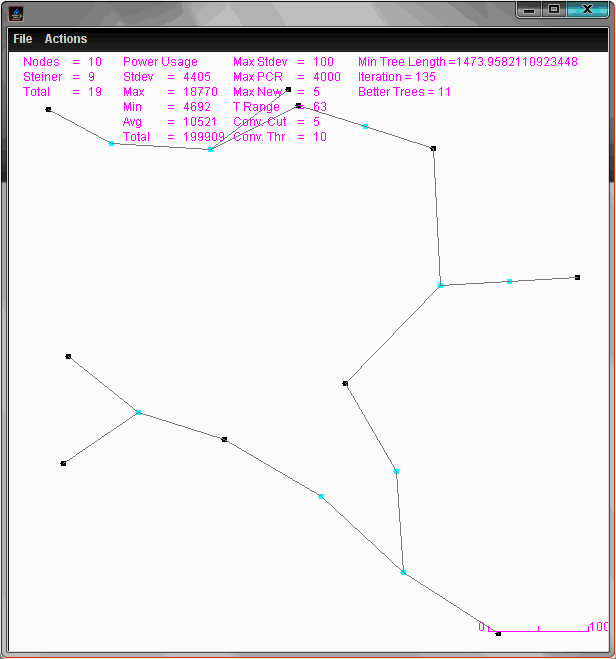
\includegraphics[scale=0.405]{images/1.PNG}
\caption{Steiner Minimum Tree Simulation.}
\label{1}
\end{figure}

A number of configurations were used to collect data.  Varied data elements include every combination of the folllowing:
\begin{itemize}
\item	Canvas size, from 100x100 pixels to 600x600 pixels, increased by increments of 100 
\item	Maximum k value, from 1 to 20 increased by increments of 1
\item	Number of terminal nodes, from 10 to 50, increased by increments of 10
\end{itemize}

Tests were run 10 times each and the results were averaged for more accurate results.  Following are graphs depicting the results, and the group's interpretation of the results.  Although it was mentioned earlier, it is worth repeating that fairness is determined by the standard deviation of the difference between power consumption rates for each node.  Therefore, the more fair a network, the lower the standard deviation. 

\subsection{Results}

Within each graph, the results are separated according to the size of the canvas on which fairness was measured.  The differences are dramatic as the canvas size increases because the distance between nodes can be much greater.

\subsection{Fairness With Varying Number of Terminal Nodes}

The following three graphs show the total power consumption for different numbers of terminal nodes.  In all three cases, the graphs confirm intuition: as the number of relay nodes increases, the graphs become more fair.  Fairness increases because there are more opportunities to minimize the difference in distances.

\begin{comment}
\begin{figure}[p]
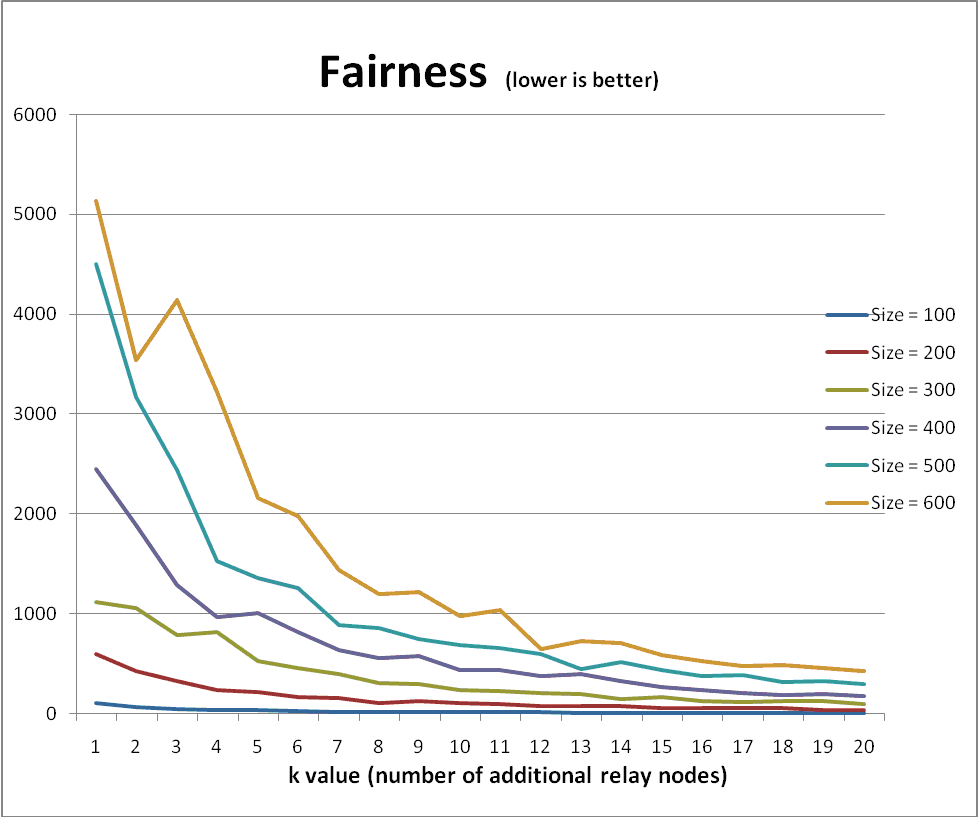
\includegraphics[scale=0.405]{images/2.PNG}
\caption{Fairness as $k$ increases; 10 terminal nodes}
\label{2}
\end{figure}

\begin{figure}[p]
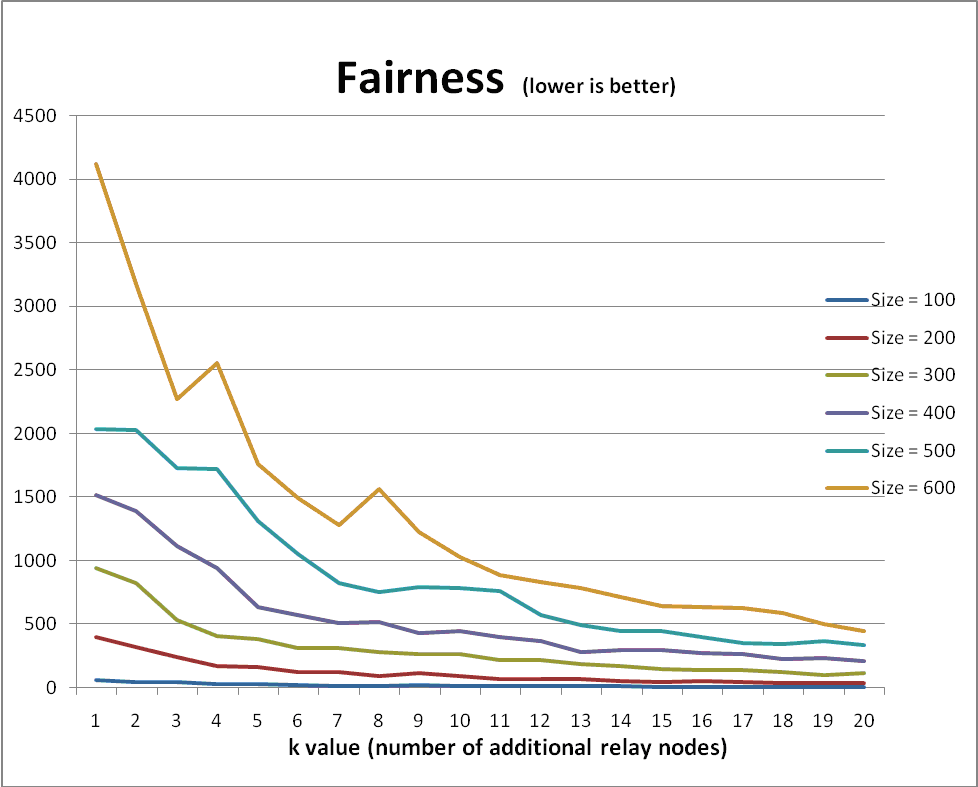
\includegraphics[scale=0.405]{images/3.PNG}
\caption{Fairness as $k$ increases; 20 terminal nodes}
\label{3}
\end{figure}

\begin{figure}[p]
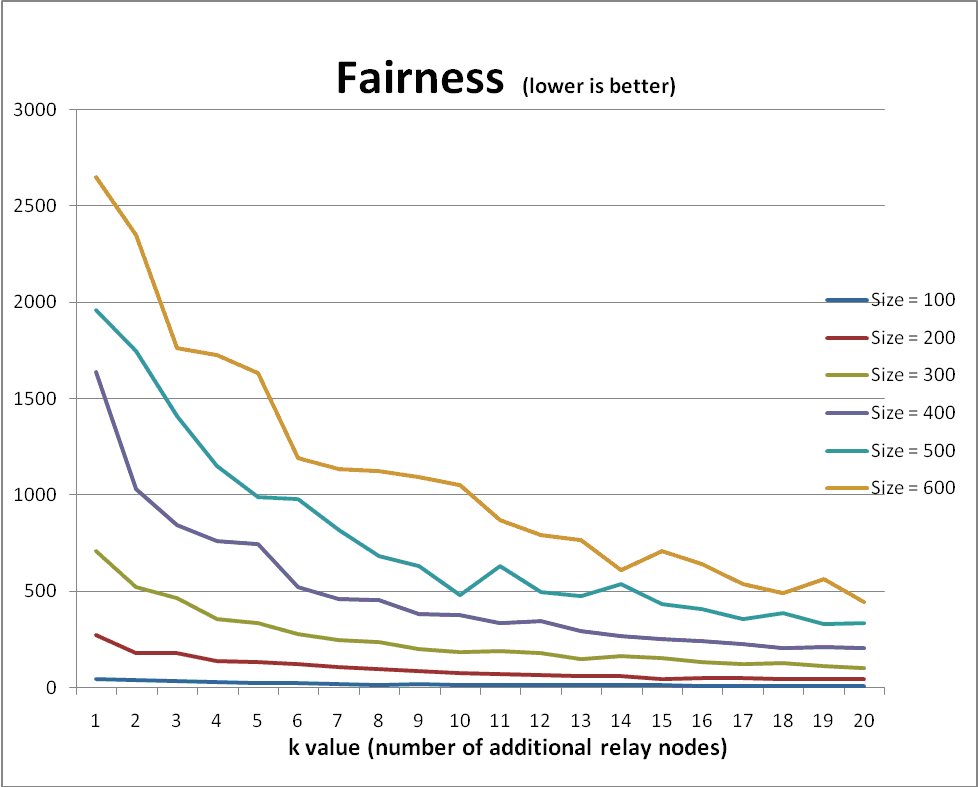
\includegraphics[scale=0.405]{images/4.PNG}
\caption{Fairness as $k$ increases; 30 terminal nodes}
\label{4}
\end{figure}
\end{comment}

Fairness is significantly different for large canvas sizes compared to smaller ones, so in order to better illustrate the trend towards fairness as k increases on small canvases, Figure \ref{5} shows a single canvas size-100x100 pixels-graphed against an increasing $k$.  As expected, it depicts increasing fairness as the number of relay nodes increases.

\begin{comment}
\begin{figure}[p]
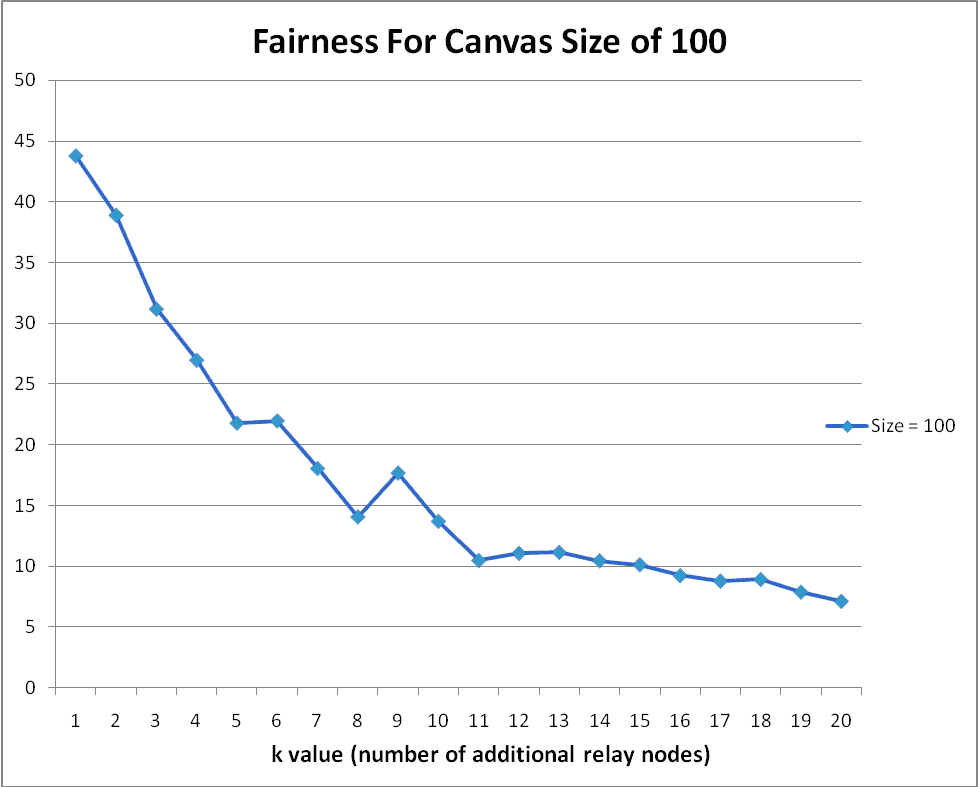
\includegraphics[scale=0.405]{images/5.PNG}
\caption{Fairness as $k$ increases; 30 terminal nodes, and a canvas size of 100x100 pixels.}
\label{5}
\end{figure}
\end{comment}

\subsection{Power Consumption}

Another interesting metric is what happens to the total power consumption as surface area increases.  As explained in an earlier section, the $PCR$ increases as distance between nodes increases.  Power consumption, therefore, decreases based on two factors: as $k$ increases, and as the surface area decreases.  Figure \ref{6} illustrates this. 

\begin{comment}
\begin{figure}[p]
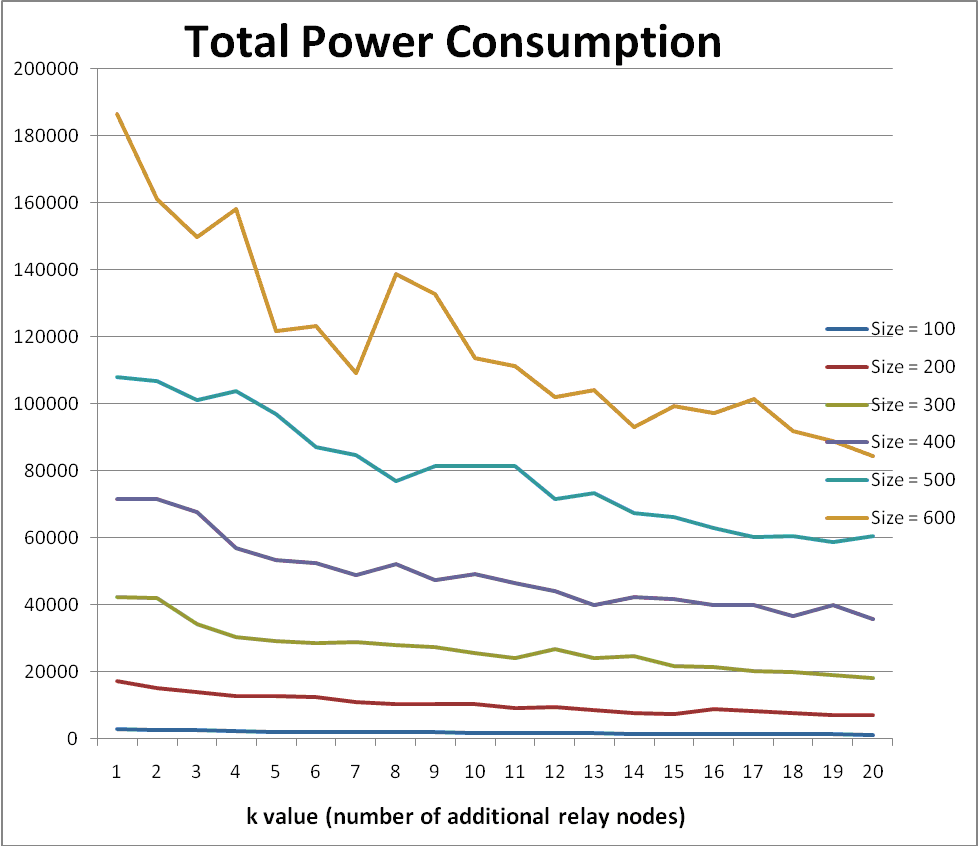
\includegraphics[scale=0.405]{images/6.PNG}
\caption{Total power consumption as $k$ increases; 20 terminal nodes.}
\label{6}
\end{figure}
\end{comment}

Total power consumption, however, is less important in the context of this paper.  More important is fairness.  To illustrate fairness in power consumption, Figure \ref{7} shows the power consumption per node on a 300x300 pixel canvas, with 20 terminal nodes, graphed as k increases.  When $k$ is low, there is little to be done to make the network fair.  By contrast, as $k$ increases, the maximum, average, and minimum power consumption per node start to converge. 

\begin{comment}
\begin{figure}[p]
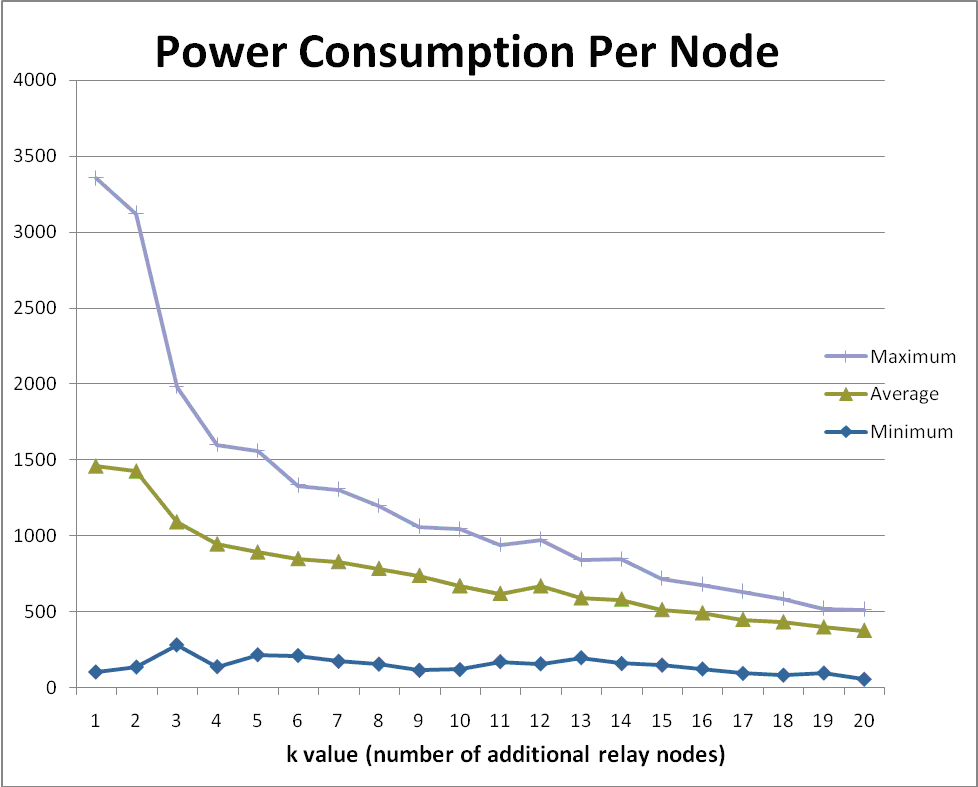
\includegraphics[scale=0.405]{images/7.PNG}
\caption{Power consumption per node on a 300x300 pixel canvas; 20 terminal nodes.}
\label{7}
\end{figure}
\end{comment}

\subsection{Interpretation of Results}

Unfortunately, the authors of this paper could not find literature studying fairness.  Consequently, it is difficult to compare the findings of this paper against some previous standard.  This section, therefore, will not compare its results with other papers.  The results of experimenting, however, do meet expectations: as relay nodes are added, fairness increases.  This is little help ultimately, as it naively implies that k should increase indefinitely.  Clearly this cannot happen: if $k$ approaches some very large number, the sensor network might as well be wired!  The problem, then, is to find a good cutoff for $k$.

\subsection{Optimal $k$ Value}

Optimal $k$ values change based on the number of terminal nodes and the surface area of the sensor network.  The graphs above and the rest of the data from experimentation show that there are very significant gains in fairness as $k$ increases from 0 regardless of the number of terminal nodes and surface area.   For networks in a small surface area, for example 100x100 to 300x300, fairness shows little gain after $k$ reaches 8 to 12 relay nodes, depending on the number of terminal nodes.  The graphs start to level off earlier when the number of terminal nodes is high, while fewer terminal nodes result in more relay nodes to reach approximate fairness.  Larger surface areas exhibit the same behavior, but require larger $k$ values before leveling off.  Although there isn't a single optimal $k$ value that fits all applications, the important aspect of the fairness is that results tend to be consistent: as $k$ increases, fairness increases, and as surface area decreases, fairness also increases.
The optimal $k$ value, therefore, should be found experimentally, given the practical constraints of the network and application.  For instance, if the surface area of the sensor network is very small, the optimal $k$ value will very likely be lower than a network with double the surface area.
